% !TEX root = main.tex
\subsection{Thrust 1: Application-Specific Trusted Execution Domains.}
\label{sb:t1}

\textbf{Problem Statement.}
Trusted execution environments (TEEs) provide an important foundation for protecting security-sensitive computation, but their trust boundaries are typically determined by the underlying platform rather than by the requirements of individual applications~\cite{mccune2008flicker,hua2017vtz,koeberl2014trustlite,brasser2019sanctuary,sun2015trustice}.
Different embedded applications, however, have fundamentally different security and resource requirements. One application may require only a processor, private memory, and access to a sensor, while another may additionally require communication interfaces, cryptographic services, or other peripherals~\cite{armanuzzaman2024building,hwang2021ambassy,teeod}.
Nevertheless, conventional TEEs often expose these applications to a fixed hardware/software trusted computing base (TCB), causing them to trust resources and privileged components that are unnecessary for their execution~\cite{schneider2020pie,gross2019breaking,cerdeira2020sok}.
This over-provisioning violates least privilege, enlarges the TCB, and increases the attack surface; in ARM TrustZone, for instance, privileged Secure-world software shares one hardware protection domain and can read all Normal-world memory~\cite{pinto2019demystifying,cerdeira2022rezone,kuhne2024aster}.

A second limitation is that the composition of the trusted environment is often not explicit to a remote verifier~\cite{lebedev2019sanctorum,nunes2019vrased,armanuzzaman2024building}.
Existing attestation mechanisms primarily establish the identity or integrity of trusted software, while the verifier must largely assume that the underlying processors, memory, peripherals, communication paths, and protection mechanisms constitute the intended execution environment~\cite{nunes2019vrased,armanuzzaman2024building}.
Consequently, verifying that the expected software was loaded does not necessarily establish that it executes within the intended hardware/software trust boundary.
The challenge is therefore not only to isolate trusted software, but also to make the resources that constitute its trusted execution environment \emph{application-specific, explicit, and verifiable}.

This thrust asks the following fundamental question: \textbf{\textit{How can embedded systems construct application-specific trusted execution domains from explicitly selected hardware and software resources, while allowing a remote verifier to establish that the intended trust boundary has actually been instantiated?}} Addressing this question requires new abstractions and mechanisms for resource specification and composition, hardware-assisted isolation, and remote attestation of the resulting domain configuration. The resulting trusted execution abstraction should be applicable across embedded architectures that provide suitable isolation and configurable resource mechanisms, rather than being tied to a particular hardware platform.


\textbf{Related Work.}
Prior work has explored more flexible trusted execution along several lines, but none makes the composition of an application-specific trusted domain remotely verifiable on off-the-shelf hardware. vTZ~\cite{hua2017vtz}, Sanctuary~\cite{brasser2019sanctuary}, TrustICE~\cite{sun2015trustice}, uTango~\cite{oliveira2021utango}, and Keystone~\cite{Keystone2020} construct multiple isolated domains by virtualizing TrustZone, partitioning memory access, running a normal-world monitor, using Cortex-M's secure attribution unit, or configuring RISC-V's PMP, respectively, but in each case the TEE and REE still time-share the same CPU and other hardware resources, leaving them susceptible to side-channel attacks rather than truly separated~\cite{armanuzzaman2024building}. CURE~\cite{bahmani2021cure}, Composite Enclaves~\cite{schneider2020pie}, and HECTOR-V~\cite{nasahl2020hector} instead grant exclusive access to specific resources -- cores, caches, or peripherals -- but all three depend on RISC-V's PMP feature or custom hardware extensions unavailable on deployed, off-the-shelf platforms. SGXIO~\cite{weiser2017sgxio} and SGX-FPGA~\cite{xia2021sgx} instead focus narrowly on protecting the I/O path between a CPU and an accelerator, rather than the composition of a trusted domain as a whole. On ARM, ReZone~\cite{cerdeira2022rezone} reduces TEE privilege by partitioning the TrustZone Secure world into zones, but relies on SoC-specific protection controllers and does not make the zone composition verifiable. Recent CCA work isolates Normal-world user-space applications (Shelter~\cite{zhang2023shelter}), relocates Android TEE services into RMM-managed Realm sandboxes with virtio-based I/O (Aster~\cite{kuhne2024aster}), or attests communication among Realms in cloud settings (Mica~\cite{sadi2026sharing}, CAEC~\cite{abdollahi2026caec}); none applies this to the Secure world or covers the platform resources (MMIO peripherals, interrupts, and DMA masters) that constitute a domain. None of these approaches makes an application's complete hardware/software trust boundary explicit, application-specific, and remotely verifiable as a single checkable property. Thrust~1 addresses this gap by treating trusted-domain composition itself as a verifiable system property.


\begin{comment}

\begin{figure}[!t]
	\centering
	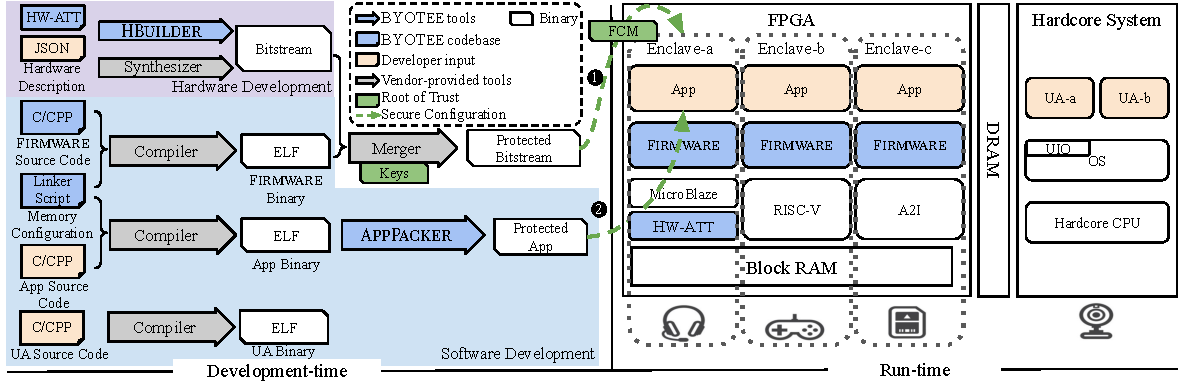
\includegraphics[width=0.98\linewidth]{figs/BYOTee-proposal.pdf}
	\caption{Preliminary foundation of \textit{Thrust 1}: \byotee{} architecture and workflow. The framework creates multiple FPGA-based hardware-software verifiable enclaves with customized  resources, firmware, and peripheral bindings.}
	\label{fig:byotee}
\end{figure}

\end{comment}

\textbf{Task 1.1: Application-Specific Trusted-Domain Composition.}
We will investigate how the security and resource requirements of an embedded application can be translated into an explicit and minimal trusted execution domain. The domain specification will identify the processing, memory, peripheral, communication, acceleration, trusted-software, and attestation resources required by the application, together with the isolation relationships among these resources. We will develop mechanisms for constructing such domains while excluding unnecessary components, unintended communication paths, and privileges that unnecessarily enlarge the trusted computing base.

\begin{wrapfigure}{r}{0.48\textwidth}
	\centering
	\vspace{-8pt}
	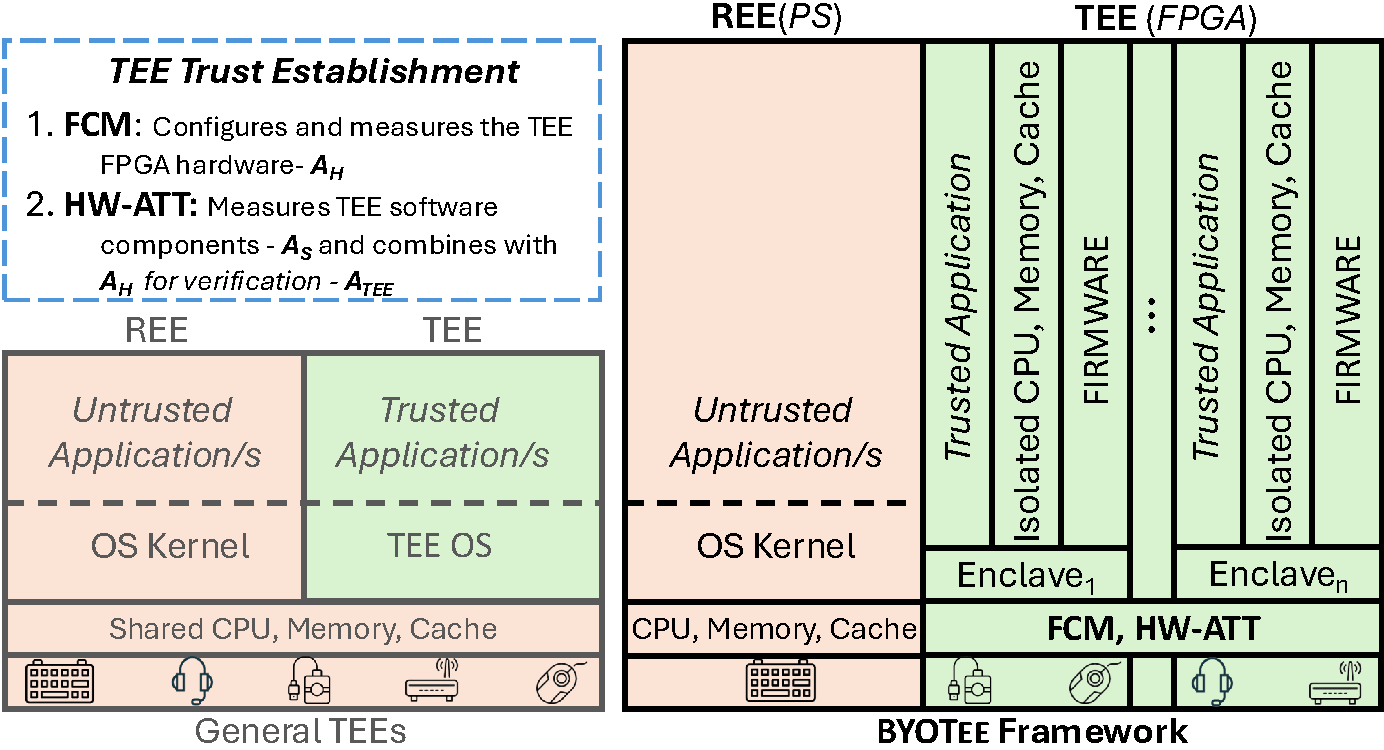
\includegraphics[width=0.48\textwidth]{figs/byotee-overview.pdf}
	\caption{Preliminary foundation of \textit{Thrust 1}: \byotee{} framework enables FPGA-based hardware-software verifiable enclave construction with resource separation.}
	\label{fig:byotee}
	\vspace{-10pt}
\end{wrapfigure}

In our preliminary work, we demonstrated this concept in \byotee~\cite{armanuzzaman2024building} on SoC FPGAs~\cite{FPGA2019}.
As illustrated in Figure~\ref{fig:byotee}, conventional TEEs typically place trusted applications within a common platform-defined boundary in which processor, memory, cache, peripherals, and privileged software may be shared across workloads.
In contrast, \byotee constructs application-specific FPGA enclaves whose hardware and software composition is determined by the requirements of each trusted application.
For each enclave, the developer specifies the required processor configuration, private memory, communication regions, peripherals, and attestation support.
\byotee then allocates and connects only the selected resources, assigns enclave-local address spaces, and generates the corresponding FPGA configuration.
Consequently, each enclave can execute with its own processor, memory, firmware, and application-required peripherals, while FPGA routing isolates these resources and communication paths from the host and other enclaves.
The software TCB is similarly minimized by including only the runtime support, hardware-abstraction components, drivers, and loader required by the protected application.

In addition to constructing the enclave, \byotee introduces two trusted hardware components for establishing the enclave configuration to a remote verifier: the FPGA Configuration Module (\textbf{FCM}) and the hardware attestation module (\textbf{HW-ATT}).
The FCM securely configures and measures the FPGA hardware realization of the trusted enclave, while HW-ATT measures the enclave software and combines the software and hardware measurements into authenticated evidence for remote verification.
Task~1.2 builds on these mechanisms to investigate verifiable trusted-domain establishment across broader embedded architectures.


\begin{wrapfigure}{r}{0.48\textwidth}
	\centering
	\vspace{-8pt}
	\begin{tikzpicture}[
			font=\tiny,
			world/.style={draw, rounded corners=2pt, align=center, inner sep=2pt, text width=1.55cm, minimum height=1.9cm},
			dom/.style={world, fill=green!14},
			arr/.style={-{Latex[length=1.3mm]}, thick},
			darr/.style={{Latex[length=1.3mm]}-{Latex[length=1.3mm]}, thick, dashed},
		]
		% ---- Normal world and decoupled Secure-world domains ----
		\node[world, fill=gray!18] (nw) at (0.8,0) {\textbf{Normal world}\\[2pt] Untrusted OS /\\ hypervisor\\[2pt] \emph{no access to\\ domain memory}\\[2pt] \textbf{Realm world:}\\ RMM unchanged};
		\node[dom] (d1) at (2.9,0)  {\textbf{Domain $D_1$}\\[2pt] SW: TA + libOS\\ Cores: $c_1$\\ Mem: $G_1$\\ MMIO: sensor\\ IRQ: 33 \\ DMA: --};
		\node[dom] (d2) at (4.65,0) {\textbf{Domain $D_2$}\\[2pt] SW: TA + libOS\\ Cores: $c_2$\\ Mem: $G_2$\\ MMIO: crypto\\ IRQ: 45 \\ DMA: $s_1$};
		\node[dom] (d3) at (6.4,0)  {\textbf{Domain $D_3$}\\[2pt] SW: TA + libOS\\ Cores: $c_3$\\ Mem: $G_3$\\ MMIO: NIC\\ IRQ: 52 \\ DMA: $s_2$};
		\draw[darr] ([yshift=3mm]nw.east) -- ([yshift=3mm]d1.west);
		\begin{scope}[on background layer]
			\node[draw, dashed, rounded corners=3pt, fill=green!5, fit=(d1)(d2)(d3), inner sep=2.5pt] (sw) {};
		\end{scope}
		\node[anchor=south, yshift=-1pt] at (sw.north) {\emph{Decoupled Secure world: least-privilege, mutually isolated domains}};

		% ---- Hardware enforcement ----
		\node[draw, rounded corners=2pt, fill=blue!10, align=center, text width=6.9cm, minimum height=0.55cm, inner sep=2pt] (gpc) at (3.6,-1.95)
			{\textbf{Hardware enforcement:} per-core GPC checks every physical access against the core's active GPT view; the SMMU checks DMA against one system-wide GPT};
		\foreach \n/\l in {nw/{V_N}, d1/{V_1}, d2/{V_2}, d3/{V_3}} {
			\draw[arr] ([yshift=-1.5pt]\n.south) -- (\n.south |- gpc.north) node[pos=0.72, right, inner sep=1.5pt] {$\l$};
		}

		% ---- Root monitor and verifier ----
		\node[draw, rounded corners=2pt, fill=yellow!22, align=left, text width=4.5cm, inner sep=3pt] (root) at (2.33,-3.7)
			{\centering\textbf{Root monitor (EL3)}\par\vspace{1pt}
			\raggedright 1.~\textbf{Build:} manifest $M \rightarrow$ disjoint GPT views $V_i$; configure MMIO, SMMU, GIC\\
			2.~\textbf{Switch:} install $V_i$ on the core (SMC); invalidate cached GPT info\\
			3.~\textbf{Measure:} $\mathbf{A}_H$ over $M$, $V_i$, MMIO, SMMU, GIC; $\mathbf{A}_S$ over domain software\par};
		\draw[arr] (root.north) -- (root.north |- gpc.south) node[midway, left, inner sep=1.5pt] {program};
		\node[draw, rounded corners=2pt, fill=violet!10, align=center, text width=1.4cm, inner sep=3pt, minimum height=1.5cm] (ver) at (6.5,-3.7)
			{\textbf{Remote verifier}\\[2pt] checks $\mathbf{A}_{TEE}$ against $M$};
		\draw[arr] ([yshift=2.5mm]ver.west) -- ([yshift=2.5mm]root.east) node[midway, above, inner sep=1pt] {nonce};
		\draw[arr] ([yshift=-2.5mm]root.east) -- ([yshift=-2.5mm]ver.west) node[midway, below, inner sep=1pt] {$\mathbf{A}_{TEE}$};
	\end{tikzpicture}
	\caption{Decoupled Secure world on ARM CCA. The Root monitor turns a domain manifest $M$ into per-domain GPT views enforced by hardware GPC and measures the realized composition as $\mathbf{A}_H$ for $\mathbf{A}_{TEE}$. Dashed arrow: declared shared window.}
	\label{fig:cca}
	\vspace{-10pt}
\end{wrapfigure}

We will extend this composition model to fixed-silicon platforms without custom or reconfigurable hardware, focusing on the Secure world of ARM CCA~\cite{li2022design}.
Today's Secure world is one hardware protection domain: the TEE OS or S-EL2 partition manager, trusted applications, secure drivers, and peripherals share the Secure physical address space, are separated only by fully trusted software, and can read all Normal-world memory.
We will develop a \emph{decoupled Secure world} in which a small Root-world monitor uses the Granule Protection Tables (GPT), which assign each physical granule to a world, and the hardware Granule Protection Check (GPC) to split it into mutually isolated, least-privilege domains, each specified by its cores, memory, MMIO peripherals, DMA masters, interrupts, and explicit channels (Figure~\ref{fig:cca}).
Because a GPT distinguishes only worlds, the monitor installs a separate GPT view on a domain's cores at each domain switch, invalidating cached GPT information; in this view only the domain's own granules and declared shared windows are accessible, so a compromised TEE OS or partition manager reaches neither other domains nor the Normal world.
Since the GPC vets physical addresses after translation, the design needs only new Root-monitor firmware on RME-capable processors and leaves the RMM, realm translation tables, and each domain's page tables untouched. It thus complements \byotee's hardware-level construction with a software-defined one on standard ARM silicon, while the domain specification remains architecture-independent.
The central challenges are (i) exclusively assigning peripherals, interrupts, and DMA masters, which the GPC alone cannot enforce (the SMMU checks DMA against one system-wide GPT and interrupts lie outside the GPT) and which prior CCA work addresses only for user-space applications and Realm VMs~\cite{zhang2023shelter,bertschi2024devlore}, (ii) preserving real-time behavior despite GPT invalidation on every domain switch, and (iii) determining whether a requested domain can be faithfully realized given residual shared state such as caches.



\begin{wrapfigure}{r}{0.48\textwidth}
	\centering
	%	\vspace{-8pt}
	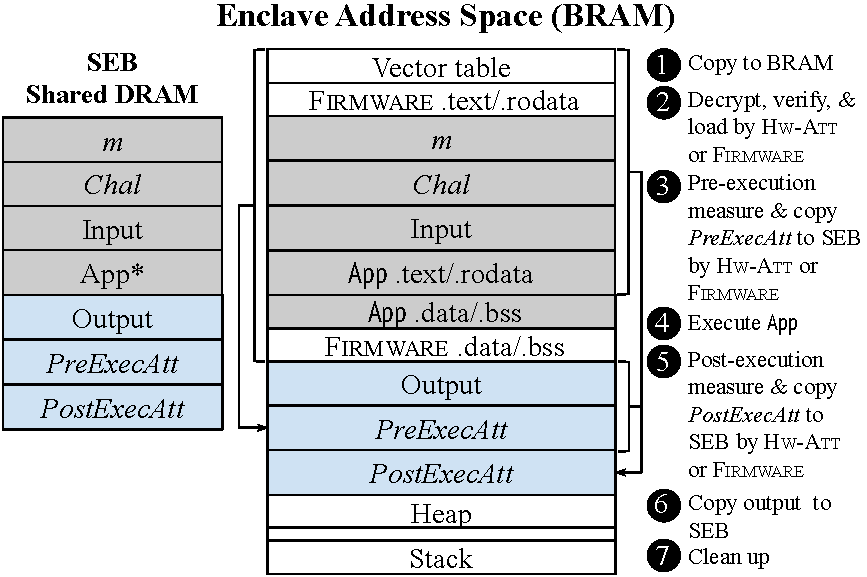
\includegraphics[width=0.46\textwidth]{figs/BYOTee-attestation-proposal.pdf}
	\caption{Verifiable trusted-domain establishment- $\mathbf{A}_{TEE}$. The FPGA Configuration Module (\textbf{\textit{FCM}}) establishes the hardware configuration measurement-  $\mathbf{A}_H$, while \textbf{\textit{HW-ATT}} measures the protected firmware- $\mathbf{A}_S$ and application for remote verification.}
	\label{fig:byotee_attestation}
	\vspace{-10pt}
\end{wrapfigure}

\textbf{Task 1.2: Verifiable Trusted-Domain Establishment.}
We will investigate how a remote verifier can establish that the trusted domain defined in Task~1.1 has actually been instantiated as intended.
Rather than attesting only the protected application, we will bind evidence about the trusted software to measurements of the security-relevant execution environment.
This will allow the verifier to determine whether both the hardware and software components of the realized domain match the expected trust specification.


In our preliminary work, \byotee~\cite{armanuzzaman2024building} demonstrates this concept on SoC FPGAs using the \underline{F}PGA \underline{C}onfiguration \underline{M}odule (FCM) and the \underline{H}ardware \underline{Att}estation module (HW-ATT), shown in Figure~\ref{fig:byotee}.
During trust establishment, the FCM verifies and decrypts the protected FPGA bitstream, configures the enclave hardware, and generates a measurement $\mathbf{A}_H$ representing the instantiated hardware configuration.
After the enclave is established, the protected application and associated firmware are loaded into enclave memory.
As illustrated in Figure~\ref{fig:byotee_attestation}, HW-ATT accesses the protected enclave memory, securely maintains attestation keys, and measures the trusted software components to produce $\mathbf{A}_S$.
The hardware measurement $\mathbf{A}_H$  and software measurement $\mathbf{A}_S$ are then cryptographically bound into authenticated evidence \textbf{$\mathbf{A}_{TEE}$} for the remote verifier.
The verifier's fresh challenge is incorporated into the attestation process to provide freshness and prevent replay of previously valid evidence.

We will generalize this hardware/software trust-establishment model to fixed-silicon embedded platforms, where the trusted-domain configuration is not represented by a single measurable bitstream.
Instead, the hardware component of the trust evidence must capture the collection of security-critical architectural states that realize the domain defined in Task~1.1, such as protection configuration, resource assignments, peripheral permissions, and execution-state controls.
On ARM CCA, this state is held by the Root monitor (Figure~\ref{fig:cca}): its granule-ownership records and GPT configuration, MMIO and DMA-master assignments, SMMU and interrupt configuration, and channel table.
Because CCA defines attestation only for the platform firmware and Realms, not for Secure-world software~\cite{kuhne2024aster}, the monitor will extend a per-domain measurement at creation and on every reconfiguration to produce $\mathbf{A}_H$, and we will investigate how to bind it to the domain's software measurement $\mathbf{A}_S$ and the verifier's challenge under the platform attestation key, with the platform's measured boot of the monitor as the trust anchor.
We will identify the minimal architecture-specific state required to construct an equivalent $\mathbf{A}_H$ across the FPGA and CCA realizations, securely bind it with the corresponding software evidence $\mathbf{A}_S$, and develop a common $\mathbf{A}_{TEE}$ representation for remote verification.
The central challenge is to ensure that evidence generated from different architectural mechanisms conveys equivalent trust semantics, allowing the verifier to determine whether the intended hardware/software domain was established across heterogeneous embedded platforms.


\textbf{Preliminary Results.}
We implemented \byotee on a Digilent Cora Z7-07S development board containing a Xilinx Zynq-7000 SoC FPGA and a 667 MHz ARM Cortex-A9 processor. Using the \byotee toolchain, we generated four application-specific FPGA enclaves with 100 MHz MicroBlaze softcore processors, private BRAM, dedicated interconnects, and selectively assigned peripherals. The generated designs demonstrate circuit-level separation among enclaves and between enclave resources and the host processor. For a digital-rights-management music-player application, the resulting runtime software TCB was only 10,727 SLOC, compared with over 117K SLOC for TF-M and 83K SLOC for the Gramine library OS as representative software TCBs for TrustZone and SGX applications, respectively. This comparison indicates the potential for substantial TCB reduction when application-specific trusted domains are used instead of general-purpose TEE software stacks. The enclave hardware and software were also measured separately by the FPGA Configuration Module and Hardware Attestation module and cryptographically combined into verifiable trusted-domain evidence. These results demonstrate the feasibility of constructing application-specific trusted domains and remotely establishing their hardware/software composition, motivating the proposed generalization to fixed-silicon embedded platforms.